\documentclass{article}
\usepackage{amsmath}
\usepackage{hyperref}
\usepackage{graphicx}
\usepackage{enumitem}
\title{COMP6252- Course work 1}
\begin{document}
\maketitle
\section{Introduction}
The goal of this assignment is to build classifiers for the music genre dataset \href{https://www.kaggle.com/datasets/andradaolteanu/gtzan-dataset-music-genre-classification}{GTZAN} using different network architectures.
The dataset includes audio samples for 10 different music genres (jazz,classical,...). Also, each audio has a visual representation constructed using MEL spectrograms.
Steps common to all architectures
\begin{enumerate}
    \item Resize the images to 180x180. This must be done when the images are loaded using torchvision.transforms.Resize. 
    \item Use PyTorch to randomly split the dataset into a training (70\%), validation(20\%), and test datasets.
    \item Run the training for 50 epoch.
    \item All the required plots should use the data downloaded from the output of TensorBoard.
  
\end{enumerate}
The above tasks should be performed for each of the following architectures:
\begin{enumerate}[label=\Alph*]
    \item A fully connected network with two hidden layers\label{q:fc}.
    \item\label{q:conv} The convolutional network shown in figure \ref{fig:conv} with your own choice of the parameters. Experiment with different parameters.
    \item Modify the CNN in figure \ref{fig:conv} by adding a batch normalization layer\label{q:bn}.
    \item Use three data augmentation methods on data and use it as an input to the architecture in part \ref{q:bn}\label{q:da}.
    
\end{enumerate} 
\begin{figure}[h]
    \begin{center}
        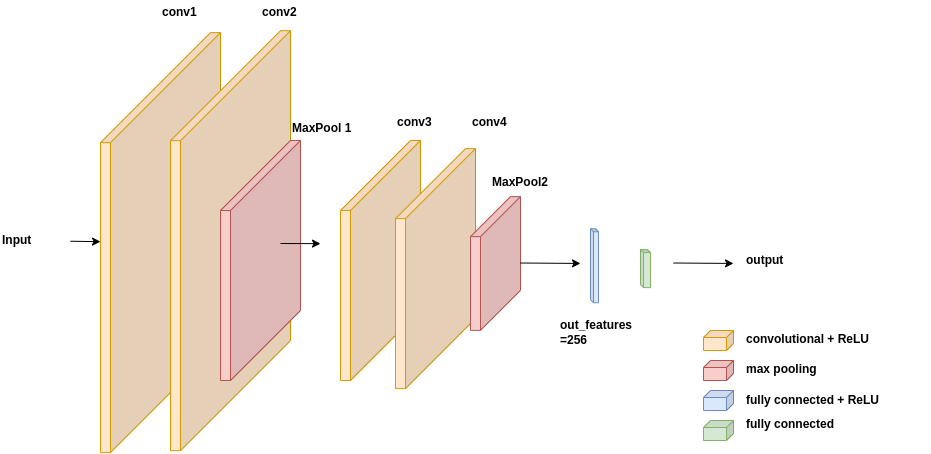
\includegraphics[width=0.9\textwidth]{course-work-conv.png}
    \end{center}
    \caption{Architecture used in part\ref{q:conv}\label{fig:conv}    }
\end{figure}
\section{Deliverables}
\begin{enumerate}
    \item A report of the results of parts \ref{q:fc}-\ref{q:conv}-\ref{q:bn}-\ref{q:da}, including 
    \begin{enumerate}
        \item The accuracy of the model on the test dataset.
        \item Plots of loss vs epoch for training and validation.
        \item Plots of accuracy vs epoch for training and validation.
        \item Plots of accuracy and loss for validation vs epoch.\label{compare}
        \item Confusion matrix for the test dataset.
        \item A discussion on the relative accuracy of the different models.
        \item Comment on the plot in part \ref{compare} 
    \end{enumerate}
    \item Discuss your choice of kernel size in part \ref{q:conv}. Include any references that back up your choice.
    \item The report must include a discussion of MEL spectrograms with the appropriate references.
    \item A \textbf{single} Jupyter notebook for all parts organized as follows:
    \begin{enumerate}
        \item The data handling, model training and model evaluation on the test data are the same.
        \item Include the network definition for all parts in sequence. E.g.: Net1, Net2,Net3
        \item It should be organized such that the only line of code that is changed to run different architectures is the instantiation of the network. E.g, model=Net1(), model=Net2(),model=Net3()
      
    \end{enumerate}
\end{enumerate}
\section{Marking}
\begin{enumerate}
    \item 
\end{enumerate}
\end{document}